\documentclass{article}
\usepackage{fullpage}

%load needed packages
\usepackage{graphicx}
\usepackage{array}
\usepackage{booktabs}
\usepackage[utf8]{inputenc}
\usepackage[T1]{fontenc}
\usepackage{hyperref}

\usepackage[spanish]{babel} % Paquete para el idioma español
\usepackage{float}  % Necesario para [H]
\usepackage{listings}
\usepackage{xcolor}

\definecolor{codegreen}{HTML}{5AB2FF}
\definecolor{morado}{HTML}{AD88C6}
\definecolor{BG}{HTML}{EEEEEE}
\definecolor{azul}{HTML}{4D869C}
\definecolor{sqlblue}{HTML}{FF8C00} % Color para las palabras clave SQL
\usepackage{listings}
\usepackage{xcolor}


%estilo python
\usepackage{xcolor}

% Define the colors for the style
\definecolor{BG}{rgb}{0.95,0.95,0.95}  % Background color
\definecolor{keywordcolor}{rgb}{0.0,0.0,1.0} % Blue for keywords
\definecolor{commentcolor}{rgb}{0.0,0.5,0.0} % Green for comments
\definecolor{stringcolor}{rgb}{1.0,0.0,0.0}  % Red for strings
\definecolor{attributecolor}{rgb}{0.8,0.3,0.8} % Purple for attributes
\definecolor{importcolor}{rgb}{0.0,0.6,0.6} % Teal for import statements

% Define the style for Python code
\lstdefinestyle{mypython}{
	backgroundcolor=\color{BG},   % Background color
	basicstyle=\footnotesize\ttfamily,  
	breaklines=true,                  
	language=Python,                  
	keywordstyle=\color{keywordcolor},    
	commentstyle=\color{commentcolor}, 
	stringstyle=\color{stringcolor},
	frame=shadowbox, 
	morekeywords={model},  % Add 'model' to keywords
	keywordstyle=[2]\color{importcolor}, % Color for import statements
	sensitive=true,       % Case sensitive
	morecomment=[s]{"""}{"} % Allows for multi-line strings
}



\lstset{style=mypython}
% Estilo para DDL
\lstdefinestyle{ddlstyle}{
	language=SQL,
	backgroundcolor=\color{BG},
	commentstyle=\color{codegreen},
	basicstyle=\ttfamily\small,
	keywordstyle=\color{azul},
	stringstyle=\color{morado},
	showstringspaces=false,
	breaklines=true,
	frame=shadowbox,
	numbers=left,
	numberstyle=\tiny\color{gray},
	captionpos=b,
}

% Estilo para SQL
\lstdefinestyle{sqlstyle}{
	language=SQL,
	backgroundcolor=\color{BG},
	commentstyle=\color{codegreen},
	basicstyle=\ttfamily\small,
	keywordstyle=\color{sqlblue}, % Color diferente para palabras clave SQL
	stringstyle=\color{morado},
	showstringspaces=false,
	breaklines=true,
	frame=shadowbox,
	numbers=left,
	numberstyle=\tiny\color{gray},
	captionpos=b,
}

\begin{document}



% Portada
\begin{titlepage}
	\centering
	\vspace*{3cm}
	
	% Título destacado
	{\Huge \textbf{Lab 1: Clustering}\\[0.5cm]}
	
	% Espacio y logotipo (si lo tienes, por ejemplo el logo de tu universidad)
	\vspace{2cm}
	
\includegraphics[width=0.3\textwidth]{images/uma_logo.jpg}\\[1cm]
	
	% Nombre del autor
	{\LARGE \textbf{Alejandro Silva Rodríguez}\\[0.5cm]}
	{\LARGE \textbf{Marta Cuevas Rodríguez}\\[0.5cm]}
	{\large \textit{Aprendizaje Computacional}\\
		Universidad de Málaga\\
		}
	
	\vfill
	
	% Fecha en la parte inferior de la página
	{\large Septiembre 2024}
\end{titlepage}

% indice
\tableofcontents

\newpage

\section{Introduction}
The process of \textbf{sporulation in yeast} is a well-established model for studying cellular differentiation and gene regulation. Sporulation involves a series of highly regulated biological stages during which the yeast cell transitions into a spore, primarily in response to nutrient deprivation. Gene expression in yeast during sporulation is characterized by distinct temporal patterns, making it an ideal candidate for clustering analysis. Through clustering, genes with similar expression profiles can be grouped, aiding in the identification of genes that may participate in similar biological functions or regulatory pathways.

With the advent of \textbf{microarray technology}, the ability to measure the expression levels of thousands of genes simultaneously across different time points has significantly advanced. This vast amount of data requires effective computational tools for analysis. One such tool is \textbf{clustering}, which groups genes based on the similarity of their expression profiles. In this context, \textbf{k-Means clustering} has emerged as a widely used technique due to its simplicity and effectiveness. The algorithm attempts to partition genes into
\emph{k} clusters by minimizing the variance within each cluster, leading to groups of genes that exhibit similar temporal expression patterns during sporulation.
\\

In this project, we aim to evaluate the performance of \textbf{k-Means clustering on the sporulation dataset} of budding yeast, comparing the results to those presented in  by Datta and Datta (2003)\cite{datta2003comparison}, which explores various clustering methods including hierarchical clustering and Diana. The primary objective is to assess the effectiveness of k-Means in clustering genes during sporulation, and to analyze how it compares to more complex methods discussed in the literature.

\section{Objectives}
The main objective of this project is to \textbf{evaluate the performance of the k-Means clustering algorithm} when applied to the sporulation dataset of yeast, which contains gene expression profiles measured across multiple time points. By clustering these genes, the aim is to \textbf{identify groups of genes} that exhibit similar expression patterns throughout the sporulation process. To assess the effectiveness of k-Means, the results will be compared to those obtained in Datta and Datta's (2003) study \cite{datta2003comparison}, which evaluated various clustering techniques, including hierarchical clustering and divisive clustering (Diana). Additionally, metrics such as the silhouette score will be used to quantify the quality of the clustering results. Through this comparison, the project seeks to determine the strengths and limitations of k-Means in clustering biological data and to explore its applicability in gene expression analysis during yeast sporulation.
	
	
\section{Methodology and Results}

We begin by preparing the environment for data processing and clustering using the Sporulation Yeast Dataset, which contains gene expression data measured at 7 distinct time points during the sporulation process. \textbf{Each row in the dataset represents a gene}, and the \textbf{columns correspond to the expression levels at different time intervals}. To focus on the relevant data, we exclude the mean and variance rows from the dataset. We designate the gene names as the Y-axis (or labels) and the time points as the X-axis (features), allowing us to analyze how gene expression levels vary over time. This preprocessing step ensures that the data is structured correctly for subsequent clustering analysis.
\\

The next step is to \textbf{normalize} the gene expression data using Z-score normalization. This method adjusts the values of each gene's expression levels to have a mean of 0 and a standard deviation of 1 across the time points. By doing this, we ensure that the expression data for each gene is comparable, preventing any gene with higher baseline expression levels from dominating the clustering process. 
\\

Now we employ the Elbow Method to identify the optimal number of clusters, 
k, for the k-Means algorithm. The Elbow Method is a well-established technique used to determine the appropriate number of clusters by evaluating the within-cluster sum of squares (also known as inertia) for a range of cluster values. 
\\

\begin{lstlisting}[style=mypython, label=fig:elbow_code,caption=Implementation of Elbow Method to the dataset]
	 
	from sklearn.cluster import KMeans
	from yellowbrick.cluster import KElbowVisualizer
	
	model = KMeans()
	visualizer = KElbowVisualizer(model, k=(2,9)) # a range of k values from 2 to 9
	
	visualizer.fit(x)        # Fit the data to the visualizer
	visualizer.show()        # Finalize and render the figure	
\end{lstlisting}


By using the KElbowVisualizer  we assess the inertia for k values between 2 and 9 as is shown in the listing \ref{fig:elbow_code}.
The visualizer generates the figure \ref{fig:elbow}.

\begin{figure}[H]
	\centering
	\includegraphics[width=\textwidth]{images/elbow.png}
	\caption{Distortion Score Elbow for KMeans Clustering}
	\label{fig:elbow}
\end{figure}



 The 'elbow' in \ref{fig:elbow}, which represents the point where the reduction in inertia starts to slow down, indicates the optimal number of clusters. In this case, the analysis reveals that \textbf{k=4} is the optimal number of clusters, suggesting that partitioning the dataset into 4 clusters strikes a balance between minimizing within-cluster variance and avoiding overfitting. 
\\

To give more information, \textbf{Principal Component Analysis (PCA)} is applied to the gene expression dataset to reduce its dimensionality from the original high-dimensional space to two dimensions. By creating an instance of the PCA class with n components=2, the code in the listing \ref{fig:pca_code} captures the most significant variance in the data while transforming it into a lower-dimensional representation. 
\\

\begin{lstlisting}[style=mypython, label=fig:pca_code,caption=Application of PCA method]
	
	from sklearn.decomposition import PCA
	import matplotlib.pyplot as plt
	import seaborn as sns
	
	pca = PCA(n_components=2)
	x_pca = pca.fit_transform(x)
	
	
	plt.figure(2, figsize=(8, 6))
	plt.clf()
	plt.scatter(x_pca[:, 0], x_pca[:, 1], cmap=plt.cm.Set1, edgecolor="k")
	# plt.scatter(x_pca[:, 0], x_pca[:, 1], c=y, cmap=plt.cm.Set1, edgecolor="k")
	
	plt.xlabel("First principal component")
	plt.ylabel("Second principal component")	
\end{lstlisting}

\begin{figure}[H]
	\centering
	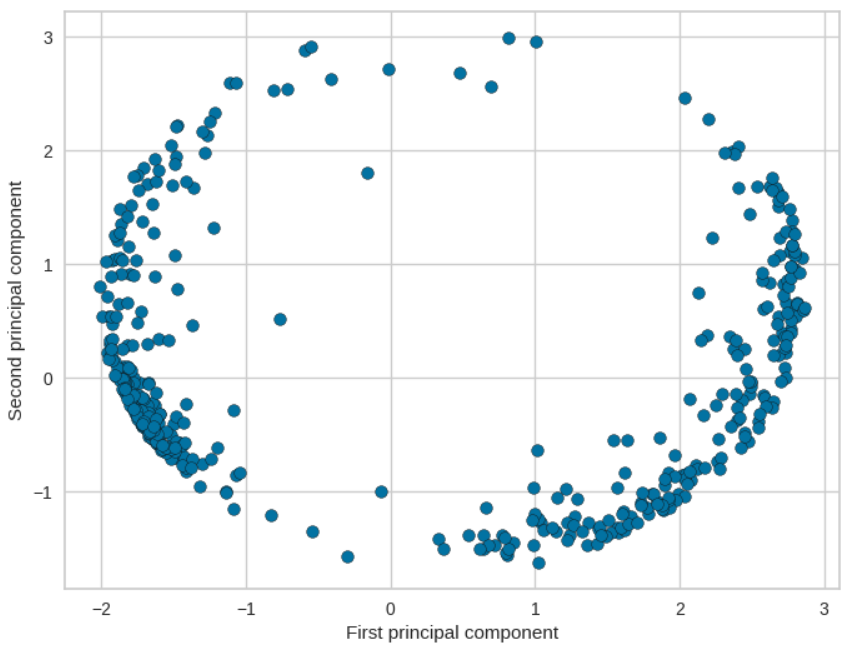
\includegraphics[width=\textwidth]{images/pca.png}
	\caption{PCA Visualization of Gene Expression Profiles During Sporulation}
	\label{fig:pca}
\end{figure}


The resulting two principal components are then visualized in \ref{fig:pca} using a scatter plot, where the x-axis represents the first principal component and the y-axis represents the second principal component. This visualization allows for a clearer understanding of the data's structure, revealing potential clusters and relationships among gene expression profiles during the sporulation process. Overall, PCA facilitates a more straightforward interpretation of complex datasets, making it easier to analyze patterns in gene expression.
\\


poner codigo de algunas cosas


imagenes y discusion con respecto a el paper

quedamos en que con nuestros datos el k=2 porque no tenemos los mismos datos que los demas. los del paper lo comparan con informacion externa que tiene mas sentido pero no es comparable con los datos de los otros ni nada.

\newpage
\section{Acceso al Repositorio}


Toda la información adicional, incluyendo el código fuente y la documentación completa de este proyecto, está disponible en el repositorio de GitHub \cite{silva2024github}.

% Incluir la bibliografía
\bibliographystyle{plain}  % Estilo de la bibliografía (por ejemplo, plain, alpha, ieee, etc.)
\bibliography{bibli}  % Nombre del archivo .bib sin la extensión

\end{document}
